\chapter{Introduction}
\label{ch:intro}     
The study of the fundamental particles is known as ``Particle Physics" for obvious reasons or ``High Energy Physics" due to the need to make observations within environments with an incredible amount of energy. On Earth this energy might be created by a particle accelerator, while in space it may be caused by the nuclear reactions in a star. Particle physics delves well beyond the fundamental building blocks of chemistry and other branches of physics which may include protons, neutrons, and photons. Over many years the existence of exotic particles bearing names with all of the letters of the Greek alphabet have been theorized and confirmed. These discoveries have been pulled together to form an outrageously successful model for describing particle interactions that nonetheless falls short in several notable instances. Modern particle physics is currently on a trajectory to test the continued limits of this model (and the many predictions it still has left to make) on the one hand, while also trying to discover what else is out there that is not described by this model. The document that follows is a description of one very small endeavor amongst many being undertaken by the thousands of people working to push the boundaries of fundamental knowledge about the building blocks of the universe. It seeks to confirm one of the, until now, untested predictions, the production of a top-antitop pair in association with a Z boson.	\\

The following discussions about the Standard Model (Ch~\ref{ch:intro}), the Large Hadron Collider and the Compact Muon Solenoid (CH~\ref{ch:LHC}), and particle reconstruction methods (CH~\ref{ch:particle_reconstruction}) lay the groundwork for the measurement performed. The remainder of this dissertation discusses the methods and details of the measurement of the \ttZ cross section as well as additional information about the combination of this measurement with other measurements of vector bosons produced in association with top-antitop pairs. The work contained in this document was performed on the data collected by the CMS detector while the LHC was colliding protons at a center of mass energy of 8 \TeV. All calculations and measurements were made with \intLumi of data. The measurement was performed to help confirm experimentally one prediction of the standard model and was chosen due to its relevance as a false positive for future works on measuring processes not predicted by the Standard Model and thus ties into the advancement of the field of Particle Physics.
	
	\section{Standard Model of Particle Physics}
	The interactions of particles with each other is described by a very accurate and far reaching theory known as the ``Standard Model." It covers electromagnet, strong, and weak  interactions and attempts to classify the known particles. It is a triumph of collaborative physics and many years of work by a very large number of experimentalists and theorists. The Standard Model (SM) was formalized more or less in the form it is now in the 1970s following experimental confirmation of the existence of quarks. But even at the turn of the 20th Century, quantum mechanical theories and extensions of it such as Dirac's Equation (which first showed that antiparticles might exist) began to feed into the body of work that became the Standard Model.\\
	
	The Standard Model is a quantum field theory that makes use of spontaneous symmetry breaking, non-perturbative interactions, and anomalies.  Standard quantum mechanics allows N to N particle interactions while field theories allow N to M particle interactions and can account for particle creation, decay, and annihilation and has managed to predict the existence of a number of particles such as the top quark and the Higgs boson. A number of partial theories existed and have been combined over the years, with the most notable being Sheldon Glashow combining the electromagnetic and weak interactions and Steven Weinberg and Abdus Salam unifying the Higgs mechanism into the electro-weak theory~\cite{halzen}.\\
	
	The Standard Model covers a wide range of particle interactions. There are 17 elementary particles (61 counting anti-particle and color variations) in the standard model (see Fig~\ref{fig:standard_particles}) with varying degrees of categorization. The highest level of categorization divides them into fermions and bosons based on their spin and other properties.
	
\begin{figure}[h]
\begin{center}
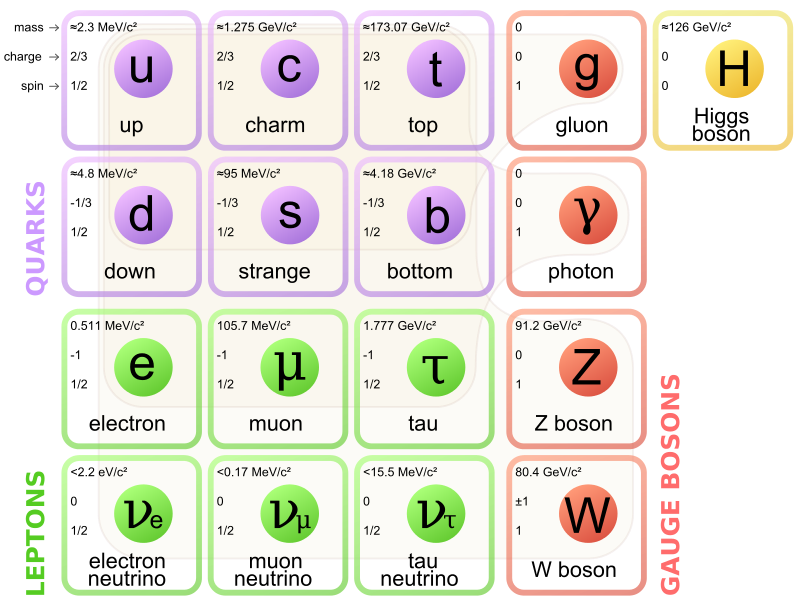
\includegraphics[width=0.8\linewidth]{Figs/Table_of_SM_particles.png}
\caption{\label{fig:standard_particles}
Quarks (purple), leptons (green), and bosons (red and yellow) are shown grouped together by their kind. Anti-particles are not shown. Quarks and leptons stacked above each other have a special relationship via the weak interactions~\cite{wikiparticles}.
}
\end{center}
\end{figure} 

\subsection{Fermions}
Fermions are spin-$\frac{1}{2}$ particles with the Standard Model fermions additionally possessing non-zero charge. The Pauli Exclusion Principle applies to these particles and their corresponding anti-particles. The fermions are further classified by their quantum numbers. The quarks have color and also possess flavor: up, down, charm, strange, top, and bottom. The leptons also have flavor: electron, muon, tau, and the corresponding three neutrinos. The particles exhibiting similar physical behavior are grouped into generations and placed in columns in Fig~\ref{fig:standard_particles} such as up and down or electron and electron neutrino.\\

Quarks primarily interact via the strong interaction with gluons as the force carrier. The theory governing quark and gluon interaction is known as Quantum Chromo Dynamics (QCD) and follows an SU(3) Gauge symmetry and is represented by the T$^a$ group with the following Dirac Lagrangian:
\begin{equation}
\mathcal{L}_{QCD}=i\overline{U}(\partial_\mu - i g_s G^a_\mu T^a)\gamma^\mu U + i\overline{D}(\partial_\mu - i g_s G^a_\mu T^a ) \gamma^\mu D
\end{equation}

They also exhibit a property known as color confinement and thus do not exist as a solitary quark for more than a short period of time. This means that they generally exist in a composite particle with two kinds existing: mesons consisting of two quarks, and hadrons consisting of three quarks. Two well known hadrons are protons and neutrons. The LHC makes use of the collisions of quarks and gluons within the protons as they pass each other in the beam pipe. Quarks also are electromagnetically charged and have weak isospin and hyper charge and thus also interact via the electromagnet and the weak interaction.\\

Leptons are the other SM fermion particles. They do not carry color charge and only interact electroweakly. Electroweak interactions are governed by a Yang-Mills Gauge theory of $U(1)\mathrm{x}SU(2)_L$ given by the following Lagrangian:
\begin{equation}
\mathcal{L}_{EW}=\displaystyle\sum_{\psi} \overline{\psi}\gamma^\mu ( i\partial_\mu - g' \frac{1}{2} Y_W B_\mu - g\frac{1}{2} \vec{\tau}_L\vec{W}_\mu)\psi
\end{equation}
Within the leptons, the neutrinos also do not carry electric charge and therefore do not interact electromagnetically. They only interact via the weak force and thus do not interact very well with our standard matter. Dedicated neutrino detectors are massive and filled with material, yet they still measure very few interactions despite a very high neutrino flux.\\

The fermions are grouped into generations and the masses of each generation are greater than those before it (again, see Fig~\ref{fig:standard_particles} with the left most lepton being the least massive). There are 12 total with all but the first generation able to decay. The first generation makes up the matter that humans interact with every day. Second and third generation quarks are short lived and decay weakly. They are only produced in high energy environments such as those at the LHC. Neutrinos do not decay and very rarely interact with matter.\\



\subsection{Bosons}
 The other types of particles in the Standard Model are bosons. Bosons are most easily differentiated from fermions by the fact that bosons have integer spin and do not follow the Pauli Exclusion Principle. The gauge bosons, that are explained by gauge symmetries in the theory, act as the force carrier that mediates strong, weak, and electromagnetic force interactions. Since it is believed that forces cannot act beyond the speed of light, and QFT requires a field for interactions, gauge bosons are considered to be exchanged between particles as they interact via the fundamental forces. See Fig~\ref{fig:sm_force_mediation} for illustrations of the interactions. 
  \begin{figure}[h]
\begin{center}
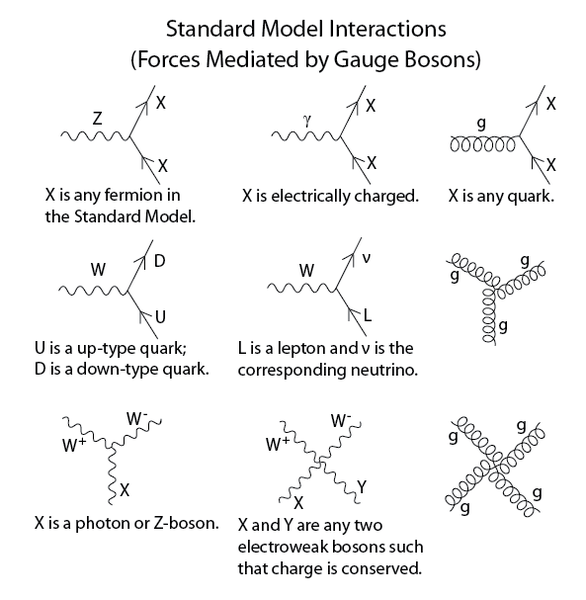
\includegraphics[width=0.8\linewidth]{Figs/SM_force_mediation.png}
\caption{\label{fig:sm_force_mediation}
 The above diagrams represent the various interactions of bosons in the standard model. As noted before a boson is considered to mediate a force between two other particles~\cite{wikimediations}.
}
\end{center}
\end{figure}
 
 \pagebreak
 
 The different SM bosons are listed:
 \begin{itemize}
 \item  Photons mediate the electromagnetic interactions between charged particles (for example electron pair production or annihilation) and are often represented with a $\gamma$. Photons are massless and thus propagate at the speed of light. They do however contain momentum equal to their energy. Photons are described by Quantum Electrodynamics which is a subset of the SM.\\
 \item There are three massive gauge bosons: W$^+$, W$^-$, and Z$^0$ with plus 1, minus 1, and neutral electric charge respectively. The W$^+$/W$^-$ are antiparticles of each other while the Z is it's own antiparticle. These particles mediate the weak interaction. The W$^{\pm}$ bosons have a mass of 80.4 \GeVcc while the Z boson has a mass of 90.2 \GeVcc~\cite{pdg}. These bosons decay quickly with the W bosons decaying to two quarks of different flavor and with opposite sign charge or a charged lepton and its corresponding neutrino. The two quarks must be one up-type (up, charm) and one down-type (down, strange, bottom). The W does not decay to the top due to mass and kinematic constraints from the much more massive top quark at current energy accelerators. For the Z boson, the decay must be to a fermion and its anti-particle which in the standard model is quarks and leptons (for example Z  $\rightarrow \ell^+ \ell^- $ where $\ell$ is a charged lepton).\\
 \item Gluons are also massless, electrically neutral particles with spin-1 which mediate interactions between color bearing particles (quarks and gluons). They exist as eight different types due to their color properties. Due to their intrinsic color charge, gluons may self interact. These interactions are described by QCD.\\
 \end{itemize} 
 

 
 The Higgs boson is the last of the standard model bosons. Unlike the previous ones, it is theorized to be a zero spin scalar, which is yet to be fully determined experimentally. It is electrically neutral and color neutral. The current best, and only, measurements come from the LHC and put the mass of the Higgs boson at 125.7 \GeVcc~\cite{discovery, higgstwiki}, which means that it can have self-interactions because it is massive. The existence of the Higgs boson is explained by a theoretical framework known as the Higgs mechanism. This mechanism exhibits spontaneous symmetry breaking and explains why the W$^{\pm}$ and Z are massive while the photon and gluon are not. Additionally the theory can explain the other mass values of the leptons and quarks. Because of the Higgs boson's special relationship with particle mass, it is far more likely to decay to the most massive particles allowed by it's current kinematic energy.\\ 
 
 
 Bosons may interact with each other as well as with quarks and leptons. These interactions are known as force carriers due to their role in propagating the various force interactions from one particle to another. See Fig~\ref{fig:boson_interactions} for the allowed interactions of the various bosons.
 
 \begin{figure}[h]
\begin{center}
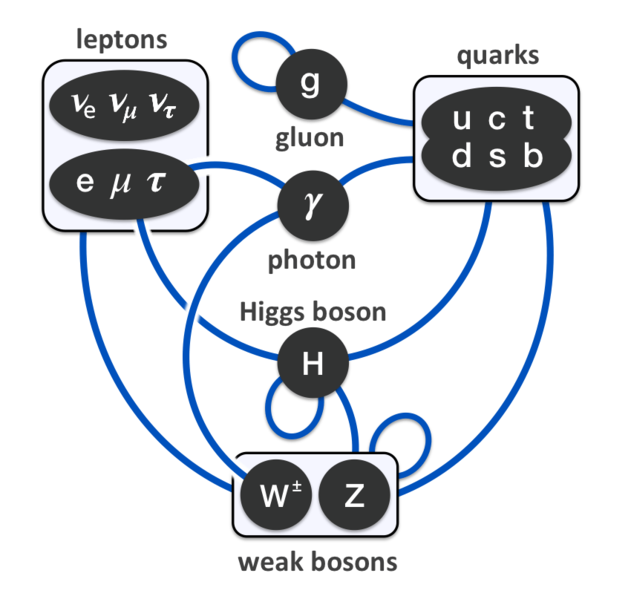
\includegraphics[width=0.8\linewidth]{Figs/particle_interactions_in_SM.png}
\caption{\label{fig:boson_interactions}
 This diagram traces the interactions between various elementary particles in the standard model. It includes self interactions as well. Lines connecting a black oval show interactions between the particles within only the two connected ovals while lines connecting a square show interactions with all of the particles within the square~\cite{wikiinteractions}.
}
\end{center}
\end{figure}

%\pagebreak

\subsection {Beyond the Standard Model}
Although the Standard Model is both a wildly successful, internally consistent theory and a highly predictive theory for particle interactions, it still is not considered complete. Experimental physics covers two branches with regard to the SM:
\begin{enumerate}
\item Higher precision measurements of known SM phenomena or new measurements of predicted but not yet measured SM phenomena. This is collectively known as SM physics.
\item Attempting to measure ``New Physics" which is physics that is not described by the Standard Model but physicists suspect exist due to deficiencies or perceived weaknesses in the Standard Model. This is primarily known as ``Beyond the Standard Model" (BSM) physics and concerns itself with things like Super Symmetry and Dark Matter.
\end{enumerate}
The topic of this dissertation is a particular Standard Model phenomena, however, the measurements of Standard Model phenomena play into the search for what else may exist that is not covered by the SM as any deviations in SM measurements from theory may provide a clue to new physics. Additionally, experimental confirmation of SM phenomena can provide helpful tools in lowering the uncertainty on BSM measurements. Thus a short explanation of what else may exist is helpful.\\

Some of the major issues with the SM are outlined below:
\begin{itemize}
\item Theories that explain gravitation's source and behavior do not have a SM description.
\item The Standard Model relies on a number of constants that do not have any clear relationship to each other in terms of values. It is considered inelegant to have such a proliferation of components that can only be measured via experiments. A complete theory would hopefully be able to relate the constants to each other mathematically.
\item One conclusion of the SM is that the weak force is much stronger than the gravitational force and leads to an excessive amount of fine tuning. This is known as a hierarchy problem and also manifests itself in the fact that the Higgs mass is many times smaller than the Planck mass. Thus the hierarchy problem is intimately tied to the Higgs mechanism (which doesn't even provide a method to calculate the Higgs mass).
 \end{itemize}
 
 Further, the Standard Model also does not answer some outstanding questions. Thus, although self-consistent, the Standard Model is not a complete description of particle interactions. Some issues are:
 \begin{itemize}
 \item Particle masses and coupling constants take on rather specific values that do not all seem to be mathematically related to each other and have only been measured experimentally. More theory is desired to provide meaningful predictions for these values.
 \item There is a matter and antimatter imbalance in the universe. There is no SM explanation for this. In fact, one would naively assume matter/antimatter to be equally abundant based on the Standard Model.
 \item Some gravitational phenomena have been observed which show that there is far more matter density in the Universe than we can see. This leads to the conclusion that there is some matter than only interacts very weakly with standard matter and has been named ``Dark Matter." There is no explanation for this in the Standard Model.
 \item There is no explanation in the Standard Model for accelerating universe expansion, or the so called ``Dark Energy." 
  \end{itemize}

As said before, these phenomena are not the topic of this dissertation. However, clear and detailed measurements of all of the SM predictions are part of the search for phenomena that are not part of the Standard Model explanation.

	\section{Proton-Proton Collisions} 
	\label{sec:pp_collisions}         
The LHC collides protons with each other at very high energies to study the resulting particles produced and ejected from the collision with the hopes that exotic particles that do not normally exist on Earth will appear briefly due to the high energy in the collision. This makes it a hadron collider. The other main work horse of particle colliders are lepton colliders. Lepton colliders provide very clean events as they only produce final state particles via electromagnetic and weak interactions. However, they are not practical for some studies at very high energies due to the difficulty posed by synchrotron radiation. A lepton collider is usually built linearly to avoid this and thus cannot take advantage of repeated cycles around a ring for continued acceleration or repeated collisions. Thus hadron colliders, though ``messier" in the products that they produce, can provide windows into physical phenomena that are not practical with lepton collisions. Additionally, they open up the possibility of a wide variety of strong interactions.\\

The probability for an interaction to occur is given by the cross section ($\sigma$), which is an analogous way to talk about the ``area" of the particles as they collide. The units typically used to measure this are barns (b) with 1 b = $10^{24}$ cm$^2$.  Due to the size of the protons, number of protons passing each other, and energy of the protons, as well as frequency of production of interesting particles such as bosons, traditionally cross sections at colliders are measured in picobarns ($10^{12}$ b) or even femtobarns ($10^{15}$ b). The average number of collisions in passing particles can be described by the equation:
\begin{equation}
\label{eq:lumi_xsec_relationship}
N = \mathcal{L} \cdot \sigma ,
\end{equation}

where N is the average number of interactions and $\mathcal{L}$ is the instantaneous luminosity (a way of measuring the amount of particles passing each other) which has units of b$^-1$.\\

At the Tevatron, the world's highest energy collider previous to the LHC, protons were collided with antiprotons. However, the LHC decided to use protons only to make production, storage, and accelerating easier~\cite{lhcmachine}. Because at its fundamental level a proton is two up quarks and a down quark (as well as some sea quarks and a lot of gluons), there is an imbalance of initial collision quarks (with up/up collisions being the most likely), whereas at the Tevatron up/antiup collisions were most likely. A typical pp crossing at the LHC has a cross section of $\sigma \approx 100$ mb~\cite{qcdprimer}. Many collisions of this type are elastic, glancing blows between two protons, and thus are not interesting to study. Some are inelastic and cause the production of new particles which are ejected and decay in the detector to study. Because inelastic collisions are between the constituent parts of a proton instead of the proton as a whole, QCD cannot calculate the energies or other meaningful properties of the resulting particles. This is due to the unknown energy and momentum of the constituent partons and how they collide. Over time, experiments have measured the range of probable outcomes of parton collisions and their frequency which can be plugged into several models to extend estimates of the probability of certain types of collisions and kinematics to conditions at the LHC. One such experiment relies on scattering electrons off of protons~\cite{halzen} and measuring the resultant debris to estimate the distribution of energy and momentum of the up, down, and sea quarks, and the gluons. Thus experimental physicists can rely on highly sophisticated Monte Carlo simulations to aid in understanding what to expect from the pp collisions at the LHC.



%	\section{Decays}
%    		(focus on boson decays to quarks and leptons to help motivate the signature later)